\documentclass{article}
\usepackage[utf8]{inputenc}

\usepackage{amsmath}

\usepackage{graphicx}
\graphicspath{{out/}}

\usepackage{float}

\title{Simple parameter estimation in the context of a Michaelis-Menten kinetic rate law}
\author{John Mason}
\date{October 2018}

\begin{document}

\maketitle

\section{Background}

This is a highly reduced basis to serve as an introduction to my broader parameter estimation work (forthcoming publication).

\section{Model}

For this demonstration, I will use a basic Michaelis-Menten kinetic rate law:

\begin{align}
v = k E \frac{C}{C + K} \label{equation:MM}
\end{align}

Note the simplified notation -- for this level of complexity, I want to avoid superscripts and subscripts as much as possible.  Here \(k\) is the catalytic rate constant, \(E\) is the enzyme concentration, \(C\) is the metabolite concentration, and \(K\) is the so-called Michaelis-Menten constant (an effective saturation constant).

\section{Objective}

Our goal is to match some target rate of reaction, \(v^\star\).  We are not considering any prior information about parameter values, so our system is not necessarily an optimization problem -- we simply wish to solve \(v = v^\star\).  For the sake of generality, however, I will express this as an optimization problem.

In this context we want the residual \(v - v^\star\) to be as small (in the sense of closeness to zero) as possible.  Thus we need to apply some metric to this residual.  For purposes that I won't expand here, minimizing the square of this residual is a practical choice:

\begin{align}
\min_{k, E, C, K} \left(v - v^\star\right)^2
\end{align}

For expressive convenience I will define \(f = \left(v - v^\star\right)^2\).

\section{The objective value space}

As previously mentioned, this problem can be solved directly via analytic approaches.  For demonstrative purposes I will instead be using graphical approaches.

Graphical approaches only work in low dimensionality space.  Unfortunately we have a function of four variables that we wish to illustrate.  This isn't an issue if we lump together parameters.

Choosing \(m = k E\) as the maximum velocity, and \(s = c/K\) as the saturation ratio, we can instead write

\begin{align}
v = m \frac{s}{s + 1}
\end{align}

This is a problem in two variables.  Thus we can now sweep \(m\) and \(s\), and plot a heat or height map of \(f\).

Another observation.  Both our original and lumped parameters are strictly non-negative values, and do tend to vary over order of magnitude.  Thus it is possible and convenient to work in logarithmically rescaled parameters\footnote{There is some weirdness about zero, since the logarithm is not finite at this limit.  In practice, this isn't terribly important, although it can lead to some numerical weirdness.}.  I defined \(\alpha = \ln m\) and \(\beta = \ln s\).  I give these no particular names -- just think of them as the magnitudes (exponents) of their corresponding lumped variables.  Now,

\begin{align}
v &= \frac{ e^{\alpha + \beta}}{e^\beta + 1}
\\ &= e^\alpha \frac{1}{1 + e^{-\beta}}
\end{align}

This new form is very nice for exploring the parameter space, as we simply need to vary \(\alpha\) and \(\beta\) linearly.  This is demonstrated in Figure \ref{figure:objective}.

\begin{figure}[!ht]
\centering
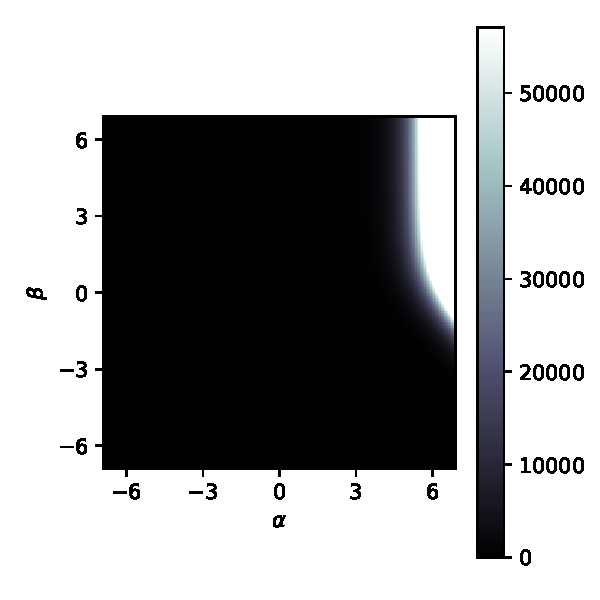
\includegraphics{figure1-raw_objective_values}
\caption{\textbf{Raw objective value sweep.}}
\label{figure:objective}
\end{figure}

Unfortunately the objective grows rapidly for large \(\alpha\) and \(\beta\).  It's easier to see the overall trend by plotting \(\ln f\), as shown in Figure \ref{figure:log-objective}.  Since \(\ln x\) is a monotonic function, this does not change the optimization problem.

\begin{figure}[!ht]
\centering
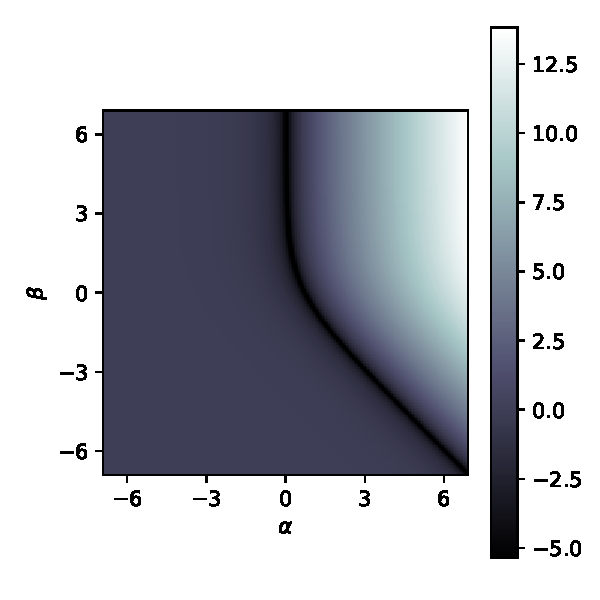
\includegraphics{figure2-log_objective_values}
\caption{\textbf{Logarithmically scaled objective value sweep.}}
\label{figure:log-objective}
\end{figure}

Now there is an obvious `valley' where the objective is minimized, corresponding to the 1D space of values for which combinations of the parameters solve our optimization problem.  Already it should be apparent that our choice of lumped parameters was more than a convenience -- for large \(\beta\), the correct choice approaches \(\alpha \approx 0\); on the other end, we have \(\beta \approx -\alpha\).

This is consistent with our knowledge about the problem.  When \(\beta\) is large, the system is highly saturated, and then all that matters is the maximum rate of reaction \(\alpha\).  In the opposite regime, near the limit of mass-action kinetics, a decrease in saturation requires a commensurate increase in the maximum rate of reaction to achieve the target rate.

\section{The gradient value space}

Most optimization algorithms are, at some level, performing a gradient descent.  Even if gradient descent can't result in a global solution, the gradient can still provide useful local information.

In our case, the gradient is just the two partial derivatives \(\partial f/\partial \alpha\) and \(\partial f / \partial \beta\).  Since \(f\) is hard to visualize, I again instead look at the gradient on the logarithm of \(f\), which is just

\begin{align}
\frac{\partial \ln f}{\partial \alpha} = \frac{1}{f} \frac{\partial f}{\partial \alpha}
\end{align}

and

\begin{align}
\frac{\partial \ln f}{\partial \beta} = \frac{1}{f} \frac{\partial f}{\partial \beta}
\end{align}

These terms are depicted in Figures \ref{figure:derivative-alpha} and \ref{figure:derivative-beta}.

\begin{figure}[!ht]
\centering
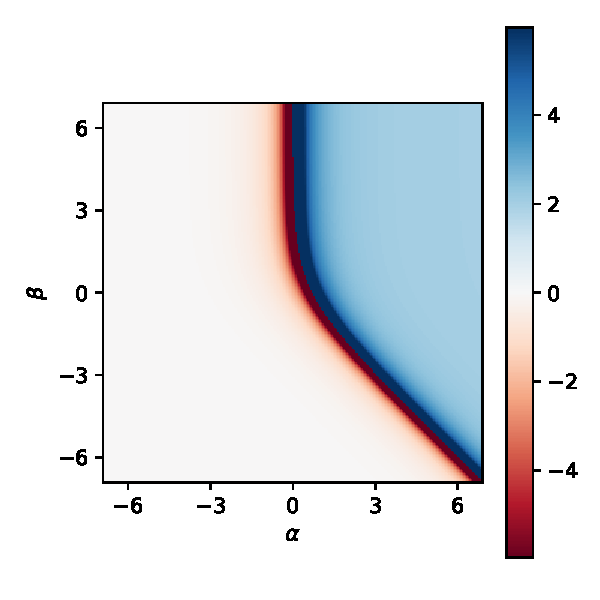
\includegraphics{figure3-derivative_alpha}
\caption{\textbf{Derivative of objective with respect to \(\alpha\).}}
\label{figure:derivative-alpha}
\end{figure}

\begin{figure}[!ht]
\centering
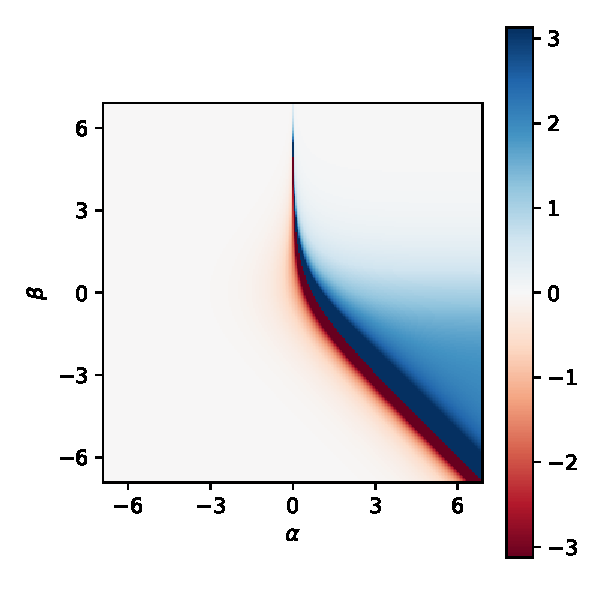
\includegraphics{figure4-derivative_beta}
\caption{\textbf{Derivative of objective with respect to \(\beta\).}}
\label{figure:derivative-beta}
\end{figure}

What we see is consistent with the analysis of Figure \ref{figure:log-objective}.  Gradients, unfortunately, are somewhat hard to interpret.  Another way to look at this is by just computing the direction of the optimal local\footnote{Note that this is not the \textit{global} best search direction, which would corrspond to snapping directly to the curved line of solutions.  In gradient descent, you're only allowed to look at the slope of the ground at your feet, so to speak.} gradient descent, as shown in Figure \ref{figure:search-direction}.

\begin{figure}[!ht]
\centering
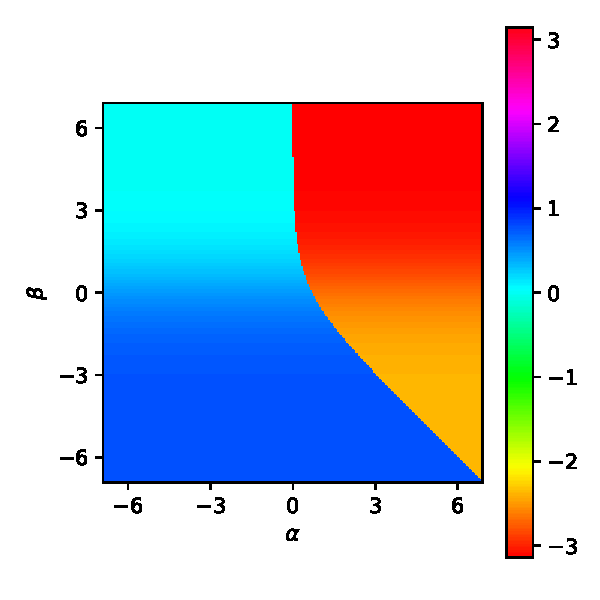
\includegraphics{figure5-best_local_search_direction}
\caption{\textbf{Best local search direction.}  The color at each point indicates the direction (in radians, with 0 corresponding to `right' and moving counter-clockwise) of the direction of gradient descent.  Roughly, `red' corresponds to `left', `cyan' corresponds to `right', `yellow-green' to `down', and `blue-violet' to `up'.}
\label{figure:search-direction}
\end{figure}

From this depiction we can clearly see that there are four regimes.  At the top these correspond to moving `right' or `left' in the parameter space, while at the bottom, the best local search direction is diagonal (up-right or down-left).  This is easier to see by looking at a flow diagram, as in Figure \ref{figure:flow}.

\begin{figure}[!ht]
\centering
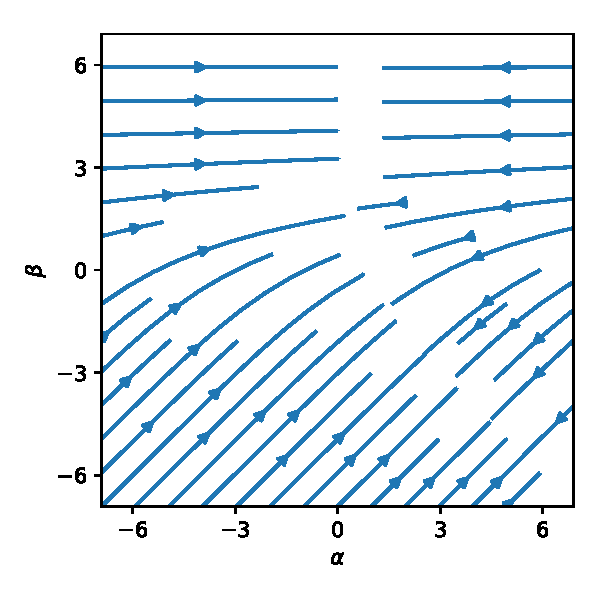
\includegraphics{figure6-gradient_descent_flow}
\caption{\textbf{Gradient descent flow diagram.}}
\label{figure:flow}
\end{figure}

The purposes of this exercise are as follows:

\begin{itemize}
	\item To develop an intuition about the parameter space, and how that corresponds to the objective space.
	\item To show how a transformation can simplify both the visualization and interpretation of the problem.
	\item To demonstrate that \(\alpha\) and \(\beta\) are a logical parameter basis for these problems.
\end{itemize}

\section{Parameter space exploration}

\(\alpha\) and \(\beta\) are not the only possible choices for lumped parameters in this model, but they probably are the best.  Remember, \(\alpha\) corresponds to the maximum rate of reaction, while \(\beta\) corresponds to the degree of saturation.  A third parameter, \(\gamma = \alpha + \beta\), corresponds to the rate of reaction in the limit of mass-action kinetics.  When divided by the enzme concentration, this term is often called the `catalytic efficiency'\footnote{For reasons, I'll add, that I don't really understand.}.  Any two of \(\alpha\), \(\beta\), and \(\gamma\) are sufficient to define this system.  Which is the `right' choice?

Let's define a few things.

\begin{align}
a &= \ln k
\\ b &= \ln E
\\ c &= \ln C
\\ d &= \ln K
\end{align}

These four new variables are just logarithms of our original independent parameters, and thus themselves are an independent parameter basis.  Now,

\begin{align}
\alpha &= a + b
\\ \beta &= c - d
\\ \gamma &= a + b + c -d
\end{align}

Already we see something critical -- \(\alpha\) and \(\beta\) are independent with respect to the underlying independent model parameters, while \(\gamma\) collides with both.  In practical terms, we can modify \(a\) or \(b\) to modify \(\alpha\) without disrupting \(\beta\), and vice-versa for \(c\) and \(d\).  Thus, even though they represent lumped quantities, we can safely claim to modify \(\alpha\) and \(\beta\) as if they were independent, as it's trivial to resolve that into changes into the underlying model parameters.  This isn't the case with \(\gamma\) and \(\alpha\) or \(\beta\).

Regardless, let's bully ahead with \(\gamma\) and see what happens.  I'm going to choose \(\alpha\) and \(\gamma\) as my lumped model parameters to explore, since they both correspond to rates (but in different model regimes).  This gives us the model equation

\begin{align}
v = \frac{1}{e^{-\alpha} + e^{-\gamma}}
\end{align}

The derivation of this form, and its graphical exploration, are left as exercises to the reader\footnote{Meaning that I've lost interest in writing any more code.  However I promise you that it has an interesting shape.}.  I do think this form is quite suggestive, given its symmetric nature.

Now, we can claim to modify these two values independently, but how do we resolve this into real parameter values if their underlying definitions are in fact interdependent?  This relation is expressed in matrix-vector form as

\begin{align}
\underbrace{\begin{bmatrix} \alpha \\ \gamma \end{bmatrix}}_{=y}
= \underbrace{\begin{bmatrix} +1 & +1 & \phantom{\pm}0 & \phantom{\pm}0 \\ +1 & +1 & +1 & -1 \end{bmatrix}}_{=\begin{bmatrix}a_1 & a_2\end{bmatrix}^\text{T} = A}
\underbrace{\begin{bmatrix} a \\ b \\ c \\ d \end{bmatrix}}_{=x}
\end{align}

This new matrix form \(y = A x\) will simplify our analysis.  Our question, more explicitly, is this: given values of \(y\), how can we find \(x\)?  This is an underdetermined problem -- which is good, but means we need some way to manage the degrees of freedom.  Taking the Moore-Penrose pseudoinverse of \(A\), we can find an \(x\) for any \(y\) as

\begin{align}
x = A^\dagger y
\end{align}

where

\begin{align}
A^\dagger = \frac{1}{2} \begin{bmatrix}
+1 & \phantom{\pm}0 \\
+1 & \phantom{\pm}0 \\
-1 & +1 \\
+1 & -1
\end{bmatrix}
\end{align}

Now, what exactly is going on here?  First off, let's note that the second column in \(A^\dagger\) corresponds to \(\beta\).  That's pretty interesting, considering that we haven't brought up \(\beta\) at all in this problem.  It fell out naturally.

How about that first vector?  Interestingly, the dot product of this vector with the vector of coefficients defing \(\gamma\) is zero -- they're orthogonal!  So, on a per-column basis, these vector represent independent means of modifying the underlying independent parameters to obtain a change in one of \(\alpha\) or \(\beta\) without changing the value of the other.

If you follow that -- and I know it's difficult -- then it's worth reexamining the case where we choose \(\alpha\) and \(\beta\) as our lumped parameters, as in the previous section.  Then

\begin{align}
A^\dagger = \frac{1}{2} \begin{bmatrix}
+1 & \phantom{\pm}0 \\
+1 & \phantom{\pm}0 \\
\phantom{\pm}0 & +1 \\
\phantom{\pm}0 & -1
\end{bmatrix}
\end{align}

These columns are just our definitions of \(\alpha\) and \(\beta\), reemphasizing their intrinsically independent nature\footnote{Perhaps it would be more appropriate to start calling these orthogonal.}.

This begins to get at the parsimonious perturabtion approach I take in my larger parameter estimtion system.  In short -- regardless of the basis taken, it's possible to explore the parameter space in a fashion that perturbs combined parameters of interest (like a maximum rate of reaction) while holding others as close to constant as possible.

What I haven't answered -- and what is, in truth, a lingering question, is which parameter space is the most natural.  The ideal parameter space would reorient the system such that perturbation to the parameters would most reliably and rapidly yield net movement towards the global (true) solution.  Apart from empirically testing alternatives, I'm not sure which choice is best.  For my current parameter estimation system, I use the equivalents of \(\alpha\) and \(\beta\), though \(\gamma\)-like parameters in place of \(\beta\)-like would be interesting to test.

\end{document}
